\documentclass[sigconf]{acmart}
% Cleaning 
\pagestyle{fancy} % removes running headers
\settopmatter{printacmref=false} % Removes citation information below abstract
\renewcommand\footnotetextcopyrightpermission[1]{} % removes footnote with conference information in first column
\pagestyle{plain} % removes running headers
\fancyhead{}
\settopmatter{printacmref=false, printfolios=false}
% Copyright
\setcopyright{none}
% \setcopyright{acmcopyright}
% \setcopyright{acmlicensed}
% \setcopyright{rightsretained}
% \setcopyright{usgov}
% \setcopyright{usgovmixed}
% \setcopyright{cagov}
% \setcopyright{cagovmixed}
\settopmatter{printacmref=false} % Removes citation information below abstract
\acmDOI{}

\usepackage{booktabs} % For formal tables
\usepackage{url}
\usepackage{algorithm}
\usepackage[noend]{algpseudocode}
\algtext*{EndWhile}% Remove "end while" text
\algtext*{EndIf}% Remove "end if" text
%\usepackage{flexisym}

\setlength{\parskip}{0pt}
\setlength{\parsep}{0pt}
\setlength{\headsep}{0pt}
\setlength{\topskip}{0pt}
\setlength{\topmargin}{0pt}
\setlength{\topsep}{0pt}
\setlength{\partopsep}{0pt}
%\linespread{0.95}
\usepackage{mdwlist}
\usepackage{amsmath}

\begin{document}
\title{Machine Translating From English to Chinese for E-Commerce Product Categorization}\titlenote{\href{https://github.com/duongy18418/Multilingual-NLP/tree/main/Code}{https://github.com/duongy18418/Multilingual-NLP/tree/main/Code}}

\author{Kitty Duong}
\affiliation{
  \institution{University of Windsor}
  \city{Windsor}
  \country{Canada}
}
\email{duongy@uwindsor.ca}

\author{Miaomiao Zhang}
\affiliation{
  \institution{University of Windsor}
  \city{Windsor}
  \country{Canada}
}
\email{zhang3s2@uwindsor.ca}

\begin{abstract}
This study explores the application of a machine translation model, Meta AI's NLLB-200, for the translation of Amazon product categories from English to Chinese. Given the critical role of accurate category translation in enhancing user experience and facilitating seamless e-commerce navigation, this research aims to evaluate the efficacy and accuracy of NLLB-200 against the existing Chinese categories on Amazon. Through a systematic translation of sample data and comparison process, the study assesses the accuracy of NLLB-200 translations, identifying both the model's strengths and its limitations in handling e-commerce terminology. The findings indicate that while NLLB-200 shows promise in accurately translating a wide range of product categories, discrepancies in certain translations highlight areas for further refinement. This research contributes to the ongoing discussion on improving machine translation for e-commerce applications and offers insights into the potential of NLLB-200 to support multilingual e-commerce platforms. The outcomes not only underscore the importance of leveraging advanced AI for localization efforts but also pave the way for future enhancements in machine translation technologies.

\end{abstract}

\keywords{Multilingual NLP, machine translation, e-commerce product categories, e-commerce translation, translation accuracy, translation evaluation}
\maketitle


\section{Problem Definition}
The global nature of e-commerce demands accurate and efficient localization of platform content, including product categories, to cater to diverse linguistic audiences. This localization is pivotal for user experience, searchability, and navigation efficiency on multinational platforms like Amazon. Traditional machine translation tools often struggle with maintaining accuracy, especially for languages with significant syntactic and semantic differences, such as English and Chinese. Introducing advanced machine translation models like NLLB-200 offers a potential solution to these challenges by promising high-quality translations across a wide range of languages, including those less represented in digital resources.

However, the effectiveness of NLLB-200 in the specific context of e-commerce, particularly for the accurate translation of product categories from English to Chinese, remains an open question. Given the critical role of these categories in user interaction and the unique challenges posed by specialized e-commerce terminology, there is a pressing need to evaluate the performance of NLLB-200. This involves not only assessing its translation accuracy compared to manually curated categories on Amazon's Chinese platform but also identifying any systematic discrepancies that could impact user experience. Addressing this problem requires a detailed analysis of NLLB-200's translation outcomes and a comparison framework that considers both direct translation accuracy and the semantic integrity of category labels.

\section{Proposed Approach}\label{approach}
Our proposed machine translation evaluation method aims to fine-tune a pre-trained model and further train it for translation from English to Chinese, then compare the accuracy of the results with the existing Chinese version on Amazon, as defined in the previous section. The approach works through two pipelined phases: the translation process and the comparison framework. In the following, we describe the details of each step.

\subsection{Translation Process}
In our approach, the translation process for converting Amazon product categories from English to Chinese using the NLLB-200 model entails preparing a standardized list of categories, setting up access to NLLB-200 through its API or SDK, and configuring translation parameters. Categories are then translated in batches, with errors and limitations managed appropriately. The resulting translations undergo initial review before being compared to Amazon's official Chinese categories to assess accuracy. The data of experiment results would be stored in a file named result.csv.


\subsubsection{Data Preparation}
In this experiment, we used the data from Amazon\_Ecommerce\_Data\_2020.csv as the dataset, which could provide a comprehensive list of Amazon product categories in English. Due to the size of the dataset, we selected around 90 pieces of data by random to test the translation capabilities of NLLB-200 across different terminologies and contexts. 


\begin{algorithm}[t]
\caption{Finding 2-d RoLs for time interval $t$}
\label{bicluster}
\begin{algorithmic}[1]
\Statex\textbf{Inputs:} 
\Statex\hspace{\algorithmicindent} users $\mathbb{U}$, topics $\mathbb{Z}$, homogeneity condition $c$, multigraph $\mathcal{G}^t$ \Statex\textbf{Initialization:}
\Statex\hspace{\algorithmicindent} $\mathcal{R}^t=\varnothing$
\Statex\hspace{\algorithmicindent} find\_2d\_RoLs($r=\mathbb{U}\times\varnothing,C=[z_1,z_1,z_2,z_2,...,z_{|\mathbb{Z}|},z_{|\mathbb{Z}|}]$)
\Statex\textbf{Output:} 2-d RoLs in $\mathcal{R}^t$
\Procedure{find\_2d\_RoLs($r=A\times{B},C$)}{}
\If{$(r\models{c})\land(\nexists{r'}\in\mathcal{R}^t: r\subset{r'})$}
\ForAll{$r"\in\mathcal{R}^t$}
\If{$r"\subset{r}$}
\State $\mathcal{R}^t\leftarrow\mathcal{R}^t\setminus{r"}$
\EndIf
\EndFor
\State $\mathcal{R}^t\leftarrow\mathcal{R}^t\cup{r}$\label{c}
\EndIf
\ForAll{$z_j\in\mathbb{Z}$}
\State $A\leftarrow{r.A};B\leftarrow{r.B\cup{z_j}};C\leftarrow{C\setminus{z_j}}$
\If{$r.B=\varnothing$} 
\State find\_2d\_RoLs($A\times{B},C$)\label{a}
\Else
\ForAll{$z_i\in{r.B}$}
\ForAll{$(z_i\rightarrow{z_j})\in\mathcal{G}^t.\mathbb{E}$}
\State $A\leftarrow{r.A}\cap{\mathbb{U}^t_{z_i,z_j}}$\label{b}
\State find\_2d\_RoLs($A\times{B},C$)\label{z}
\EndFor
\EndFor
\EndIf
\EndFor
\EndProcedure
\end{algorithmic}
\end{algorithm}



\begin{figure}[t]
\centering
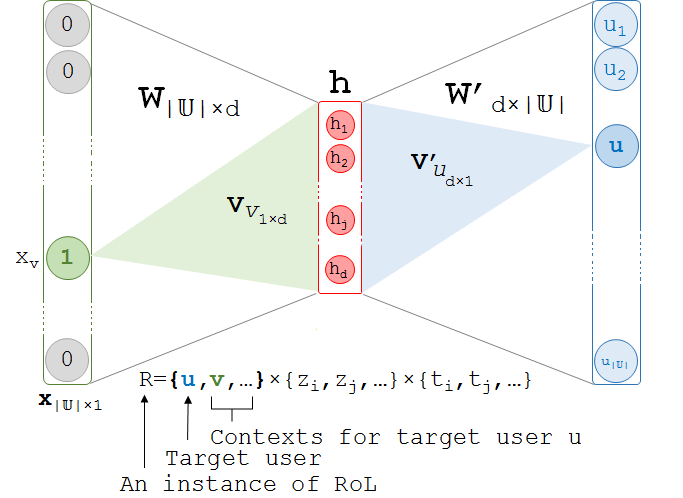
\includegraphics[width=0.8\columnwidth]{Images/neural_net.png}
\caption{The neural network architecture.\label{neural_net}}
\end{figure}

\subsubsection{Fine-tune NLLB-200 Model}
We utilized the API provided by MetaAI to set up an environment for accessing the NLLB-200 model. Besides, we followed the tutorial from Hugging Face to use PyTorch Trainer to finetune the pretrained model. Based on the configuration settings to specify source (English) and target (Chinese) languages, we sent batches to NLLB-200 for translation processing.

\subsubsection{Post-Translation Processing}
As for the experiment results, we stored the translated categories alongside their original English counterparts in a file name result.csv for further analysis. We could review the translated categories for initial quality assurance. 

\subsection{Comparison Framework}
This comparison work would focuses on semantic equivalence and terminology appropriateness between the experiment results and the existing Amazon Chinese version. Furthermore, discrepancies are documented, and a statistical analysis is conducted to evaluate NLLB-200's overall performance, aiming to highlight the model's strengths and areas for improvement in e-commerce localization.

\bibliographystyle{ACM-Reference-Format}
\bibliography{bibliography.bib} 

\end{document}

